\documentclass[12pt]{article}
\usepackage[SlantFont]{xeCJK}
\usepackage{fontspec}
\usepackage{cite}
\usepackage{amsmath}
\usepackage{graphicx}
\usepackage{booktabs}
\usepackage{pgfplots}
\usepackage{caption}
\usepackage{subcaption}


\setCJKmainfont[BoldFont = SimHei]{SimSun}
\setCJKmonofont{SimSun}

\title{论文图片中定位行内公式}
\author{张浩然 1500010684 \\ 北京大学~数学科学院~信息科学系}
\date{} 

\begin{document}
\bibliographystyle{plain}

\maketitle
\tableofcontents

\newpage
\abstract{公式是我们在论文中比较关心的对象,而行间公式在很显著的位置,行内公式则不容易快速分辨。将论文图片中的行内公式快速定位并识别,是一件有意义的事情。若把这看作一个目标检测的问题,则可以使用经典的目标检测算法去解决这个问题。又或者以这个问题的特殊性为基础,先做图像预处理,进行单词分割,再使用分类器对单词图片进行分类,选出公式图片。这篇文章使用了一系列基础的图像处理手段并用神经网络作为分类器,参考了一些复杂的模型来提高性能。}

\section{背景介绍}
\noindent

现在的论文多以pdf格式或图片格式进行传播,在使用这些论文时,其中的公式部分往往是我们关心的地方,而快速找到并获取其中的公式就成了一项有意义的工作。我们在这里试图利用神经网络来解决论文图片中公式定位这个问题。

在处理论文图片中定位公式位置这个问题上,我们准备了两个方向上的方法。一是将论文图片切割为段落图片后使用目标检测方法来定位公式的位置,二是在预处理上更进一步将论文图片切割为单词图片,再将单词图片分类。

在目标检测这个问题上有许多的经典算法。基于卷积神经网络的目标检测开始于2013年RBG的论文\cite{rcnn}提出的RCNN。RCNN的算法过程大致为生成候选区域后使用CNN进行特征提取,将提取的特征通过SVM分类,最后通过边框回归(bounding-box regression)得到精确的目标区域。此算法的主要问题在于候选区域过多,大量的区域重复和无效造成了巨大的计算浪费。另一个问题在于使用CNN需要输入固定尺寸的图片,而图片的截取和拉伸等操作造成了输入信息的丢失。之后有许多算法以此为基础进行了改进。

首先是空间金字塔池化SPP-Net\cite{spp},在全连接层前加入了一层将输入的特征图池化为特定尺寸的输出的特殊池化层,通过输入的尺寸与需要的输出尺寸计算出所需的池化核和步长从而实现了输出固定尺寸至全连接层。而之前的卷积层并不依赖于输入图片的尺寸,从而实现了任意尺寸的输入。实际上是将原图片多尺度采样输入带SPP层的CNN进行训练,也是被称为金字塔的原因。

之后RBG又提出了新的Fast-RCNN\cite{frcnn},借鉴了SPP的思路提出了ROI池化层,以及将SVM分类改为使用softmax进行分类,并将分类和边框回归整合,不再独立进行训练。这个算法将除了候选框提取的所有步骤整合在一起进行训练,并引入类似SPP的池化层解决了不同尺寸的输入问题,使得训练过程大大提高了。

之后Faster-RCNN\cite{ftrcnn}又更进一步,提出了RPN解决了候选框提取的问题。RPN的特点在于不是在原图上进行候选框提取,而是在特征图上进行。原图通过CNN后首先在特征图上进行候选框提取,并将候选框进行分类,只将感兴趣的区域输入到ROI池化并进行下一步的分类学习。这样做可以让网络自己学习生成候选区域,大大减少选取候选区域的冗余,提高了预测时间,使得预测可以做到实时。至此候选框选取,CNN,ROI池化,分类与边框回归都整合到一起训练。

YOLO\cite{yolo}则使用了另外一个思路,直接将整个图像进行训练,不预先进行候选框提取。将整个图像分为$S \times S$的网格,物体的中心所在的网格负责该物体的检测,直接经过神经网络得到输出,输出包含物体位置、类别和置信度信息。YOLO全称为You Only Look Once,体现了该算法的简介和迅速。该算法相对于RCNN系列的算法拥有检测速度快和背景误检率低等优势,但在准确率和物体位置精度上较差。而且YOLO只在一个网格尺度上进行回归,缺乏多尺度信息,容易丢失小目标。

SSD\cite{ssd}在YOLO之上做了许多改进,采用了多尺度特征图的检测来适应不同大小的物体,最后的输出不是使用全连接层而是用卷积来取得检测结果,同时引入了Faster R-CNN中anchor的概念,设置不同长宽比和尺寸的先验框。这些改进使得SSD同时获得了较高的准确率和速度。

除了使用目标检测的方法,另一方面从单词切割入手,提前获得单词的位置,再将单词图片利用CNN分类。我在这个方向上自己写了具体的代码实现,下面对这个方法进行详细的叙述。



\section{数据处理}

\subsection{tex文件到图片}
\noindent

我们首先从网上获得了大量的论文tex文件,通过正则表达式找到其中被\$...\$框住的公式部分,由于我们的关注点只在于行内公式,故被\$\$...\$\$框住的行间公式部分需要排除,找到后在公式外加上可以框住公式的LaTeX命令,并分为使用红框和使用白框两个版本。使用白框的是我们进行训练的主要数据,红框版本是获得标记使用的。为了支持我们新增的LaTeX命令,仍需要使用正则表达式检测是否含有我们需要的宏包,若没有则在开头加上。接着将处理完毕的tex文件编译为pdf文件,在编译过程中发现大量的编译失败,主要原因一是使用的tex文件较为久远,主要为2001-2003年的数据,编译格式和使用的宏包各种各样,缺少相应的宏包支持,二是文件的编码格式不是utf-8,而编译时统一以utf-8为标准,故导致了读取失败。成功编译的pdf中也有少量缺失正文,只有公式存在。而且由于为了迅速编译,故所有文件只进行了一次编译,这样所有的引用都不会生效,参考文献的编号都变成了?,认为不影响本工作,所以忽略不需解决。

然后是将pdf文件转化为png图片。由于预计使用工具magick来进行转化,而为了全程使用python编程,故使用了magick的python包PythonMagick,而此包缺少文档说明,故一开始转化为png时遇到了困难,故一开始使用的是jpg格式。在查阅了许多解决方法后才终于得到了png文件,发现相同尺寸下png格式的图片只有jpg格式的几分之一,大大减小了硬盘占用,加快了数据传输。

以上方法都写在了文件texf\_topng.py中。宏包使用了re, os, pdflatex, PythonMagick, PyPDF2, 并导入了自己写的图片处理工具文件。re为使用正则表达式的宏包,pdflatex是将tex编译为pdf的宏包,PythonMagick是将pdf转化为png的宏包,PyPDF2是辅助pdf分页生成图片的宏包。在生成图片的同时裁去了图片的空白边框并通过生成的图片是否有红框来删去了不带公式的图片。单个tex文件处理使用文件ttp.py,批量文件处理使用ttpb.py。通过以上方法生成了红框版本和白框版本共计16万张图片,每张图片的生成速度在一秒以内,实际生成时使用并行处理。本方法由于还要将论文图片分割为单词,故实际使用的图片数没有这么多。

\subsection{单词分割及数据预处理}
\noindent

单词分割主要分为两个部分,文行分割与行内单词分割。以下处理均使用灰度图像。行和是指图像矩阵一行中非空白元素的比例,由于提前做了图像反转,白色为0,黑色非零,故只需要将一行二值化后求和除以列数,故称为行和。文行的中心行和指文行中间一行的行和,同理,开始行和和结尾行和指文行开始行和结尾行的行和。

在处理之前首先判断图片方向,认为一般只有正向和逆时针90度方向。由于灰度图像白色为255,黑色为0,故先将图片矩阵反转为白色为0,黑色为255,再分别求得图片矩阵的行和和列和。如果图象是正向的,空白边框也已经被截去,故认为行和中0的比例应大于列和中0的比例,因文行和文行之间有固定的空白,而单词与单词之间的空白位置每行不一。以此作为是否要将图片旋转的依据。此判断只对整页论文有效果,若进行单行或单个单词测试则无效,故设置为可以关闭。

文行分割这个问题上,文行与文行之间有明显的空行,以空行作为文行的边界即可。由于只关心行内公式,故文行分割还有更多的要求,需要在分割时排除行间公式和一些特殊的文行,如一条直线、图表、页码、特殊符号等。故以空行作为边界分割后,又以中心行和,前四分之一行和,开始行和,结尾行和和行高度作为标准来去掉不符合需求的文行。行间公式和一条直线这种情况,一般高度与正常的文行有差别,行间公式大部分高度比较大,一条直线、特殊符号等则是高度比较小,故筛选出高度在平均高度一定范围内的文行。而页码则是中心行和极小,实际上行间公式的中心行和也小于正常文行的行和。同时行间公式的前面通常是一片空白,故同时使用前四分之一中心行和来同时作为辅助标准。为开始行和和结尾行和则是为了去掉图表。

文行分割后,就是对每一文行进行单词分割了,我们使用的都是英文文档,故这里只考虑英文的单词分割。同样预先进行图像反转,使得白色为0,黑色非零。单词分割与文行分割有相似之处,同样是利用单词与单词之间的空白。但容易注意到一行内的空白有三种情况,单词与单词间的空白、字母与字母间的空白和另外一些比较大的空白,如一行结尾后还有大片空白,每段开始文行的开头空白等。这些空白的位置使用列和就可以轻易找到,接下来就是在这些空白中筛选出单词间空白。由于最后是利用空白的位置来分割出单词,故认为大片空白和单词间空白是同一性质。这里使用的是最小二乘法,找到使得公式最小的空白宽度,然后认为在这宽度以上的都是用来分割单词的空白。这样做的效果还不错,大多数单词都可以分割出来,少数情况下会出现一个单词被分为两个,而常见的情况是一个长公式被分割为多个单词。

以上单词分割不仅可以分割出单词图片,同时可以获得分割出的文行的位置和每个文行中每个单词的位置,结合去除空白边框时获得的左上角的非空白元素的位置,可以将每个单词的位置精确地还原。

将白框版本的图片进行了单词分割,获得了单词图片及其位置,在通过其位置信息在红框版本的图片中检查该单词是否被红框框住,以此获得每个单词的标注。这样我们将原本的图片整理成了单词图片、单词位置信息和单词标注信息,训练神经网络只需要单词图片和标注信息,故将这部分做成tfrecords文件以备后续使用。由于一张论文图片中非公式单词比公式单词要多得多,故这里采用了过采样,将公式图片直接复数拷贝,使得公式图片与非公式图片的数量接近。过采样后实际使用的单词图片为100万张左右。

\section{网络结构与算法}

\subsection{激活函数与损失函数}
\noindent

神经网络中有两个重要的部分,一个是激活函数,一个是损失函数。激活函数是实现网络非线性化的重要手段,常用的激活函数有sigmoid函数、tanh函数和ReLu函数等。其中sigmoid函数和tanh函数由于当输入比较大时会有梯度接近0的问题,即梯度消失,使得非监督训练的效果较差。ReLu函数如下:
$$relu(x) = 
\begin{cases} 
0& x < 0\\
x& x \ge 0
\end{cases}$$
ReLu有计算简单迅速而且不会有梯度消失问题的优势。ReLu仍有些问题,一是若训练发散,会迅速增大或减少到nan,使得结果报错。故开始训练前应仔细检查网络的设置,确保能够收敛。二是ReLu函数将小于零的值直接变为0,使得该输出都为正值,故可能会造成某些神经元的失活,不管怎样训练都为0。同时ReLu的输出都为正值,使得收敛比较困难。故针对ReLu有许多的改进的函数。Leaky ReLu函数为在ReLu的基础上,在$x<0$时加上一个较小的斜率。PReLu则是使得这个斜率作为一个可以训练的参数加入网络中,RReLu的做法则是将这个斜率根据均匀分布随机抽取。PReLu的输出更近接近0,收敛速度比ReLu更快,故我使用的是PReLu。

分类问题使用的最普遍的的损失函数是交叉熵函数$$- \sum_x p(x) \log q(x)$$ 要使用交叉熵函数需要输出和目标都满足概率分布,故交叉熵函数一般结合softmax函数$$softmax(y)_i = y'_i = \frac{e^{y_i}}{\sum^n_{j=1} e^{y_j}}$$将输出和目标都归一化。在二分类时也可以使用sigmoid函数$$sigmoid(y) = \frac 1 {1 + e^{-y}}$$将输出转化为$[0, 1]$之间作为概率使用。在二分类时,softmax的表达式为$$softmax(y)_1 = \frac{e^{y_1}}{e^{y_1} + e^{y_2}} = \frac 1 {1 + e^{y_2 - y_1}}$$ 故神经网络输出的两个值的差与只输出一个值是等价的,差别在于前者的全连接层会有更多的训练参数。我实际使用的是sigmoid函数。

\subsection{神经网络优化算法}

\subsubsection{指数衰减学习率}
\noindent

神经网络的学习率代表神经网络参数的更新速度,较大的学习率使得参数每次更新的幅度较大,收敛得更快,但可能会导致无法收敛到最小,每次更新的时候都跳过了能够收敛到最小值的范围;学习率太小又会导致参数更新太慢,网络收敛速度太小。一般而言,开始时希望学习率比较大,使得网络快速收敛,然后学习率逐渐降低,使得收敛更为准确。故使用了如下阶梯状指数衰减学习率,将学习率乘上一个指数衰减率,使得学习率随着训练次数逐渐降低。实际为每学习1000轮将学习率乘以0.9。

\subsubsection{批标准化batch normalization}
\noindent

神经网络中的数据在经过每层的处理后数据分布可能会发生变化,这一过程被称为Internal Covariate Shift\cite{bn}。这种数据分布的变化传递到后层网络中,后层网络也需要不停地去适应这种分布的变化,这就导致了网络的收敛速度下降。如果采用的是饱和激活函数,如sigmoid或tanh,数据分布变化会导致数据变大进入梯度饱和。而如果是ReLu激活函数,则会有数据分布差异大,深层网络收敛困难的问题\cite{bn-relu}。

由于以上问题,我们使用了batch normalization方法,即对每层的数据做规范化。对一层中的一批数据的每个通道$\{x_i : 0 \le i \le n\}$,做如下规范化操作
$$\mu = \frac 1 n \sum^n_{i = 1} x_i$$
$$\sigma^2 = \frac 1 n \sum^n_{i=1}(x_i - \mu)^2$$
$$\hat{x}_i = \frac{x_i - \mu}{\sqrt{\sigma^2 + \epsilon}}$$
$\epsilon$是为了防止方差为0。这样规范化后每一层网络的数据分布都变得稳定,但数据的表达能力却缺失了。为了获得原有信息,BN又引进了两个可以在网络中进行学习的参数$\gamma$和$\beta$,使得规范化后的数据可以通过变换$\tilde{x}_i = \gamma \hat{x}_i + \beta$恢复表达能力。当$\gamma^2 = \sigma^2, \beta = \mu$时,$\tilde{x}_i = x_i$,即是完全恢复为原来的数据。这样我们既使得每层的分布变得稳定,又能够保证数据的表达能力。规范化是在一个batch的每个通道上做,而偏置项对于一个通道而言是相同的,故只需要对卷积输出做规范化,然后加上偏置项就可以了。

BN使得网络的每层数据的分布变得稳定,后层网络不必去适应输入的变化,实现了每层的独立学习,提高了整个网络的学习速度。在使用ReLu激活函数时,由于ReLu函数的输出都非负,故输出平均值远离0,网络不容易收敛,若不使用BN,使用MSRA初始化30层以上的网络也难以收敛\cite{bn-relu}。同时BN处理后,将降低网络中的参数的敏感度,使得调参,如初始化、学习率等的设置更为容易,不用担心参数的变化随着网络层数加深被放大。使用BN后,也不用担心数据经过多层网络后落入饱和性激活函数的梯度包和区,从而可以缓解使用sigmoid,tanh等激活函数的梯度消失问题。同时BN并没有完全保留原始数据的信息,而是通过学习参数$\gamma, \beta$来一定程度上保留数据的表达能力,这就相当于给数据加入了随机噪音,可以起到正则化的效果,防止数据的过拟合。在原作者的结果中,BN可以在没有dropout的情况下同样达到很好的泛化效果,而且网络的收敛速度提高了很多。\cite{bn}我在网络中也同样使用了BN。

\subsubsection{滑动平均}
\noindent

滑动平均,或指数加权平均是一个使得神经网络模型在测试数据上更加健壮(robust)的方法,在计算网络输出时,使用的网络模型不是当时的模型,而与一段时间内的历史模型有关。变量$v_t$在更新为$t$时刻的取值$\theta_t$时,使用公式
$$v_t = \beta v_{t-1} + (1 - \beta) \theta_t$$
上式中$\beta \in [0, 1)$,$\beta$一般取值较大,即变量在更新时使用了上一时刻的取值,做了某种平均,这样不需要保存一段时间内的每个网络就可以获得某种网络的均值。在网络训练的后期,网络会在在一定范围内波动,使用滑动平均后的网络变量来测试数据就能提高测试结果的表现和稳定性。注意到在网络训练的前期我们希望模型可以更新得更快,故希望衰减率较小,来使得变量快速学习更新。Tensorflow提供了tf.train.ExponentialmovingAverage函数来实现滑动平均,还提供了参数num\_updates来实现动态设置衰减率的大小,使得网络前期衰减率较小,可以快速学习更新,训练到一定程度后则使用较大的衰减率来实现更好的滑动平均。

\subsubsection{过拟合优化}
\noindent

大规模的神经网络有一个重要的难题存在,那就是容易过拟合。神经网络在学习中容易过度学习训练数据的特征,将数据中的噪音也一起学习下来,从而在测试集上的表现效果和训练集上差异较大。

处理过拟合有许多的方法,其中上述的BN就能在一定程度上取得效果。另外一个常用的方法是正则化。正则化是在损失函数后加上一个刻画模型复杂度的函数。
$$J(\theta) = J_0(\theta) + \lambda R(w)$$
$\theta$代表神经网络中所有要学习的参数,$w$表示网络权重,$J_0(\theta)$代表原损失函数,$R(w)$使用中对网络复杂程度的刻画,$\lambda$为模型复杂损失在总损失中的比例。再使用优化算法,如梯度下降时,不是直接优化$J_0(\theta)$,而是同时优化$R(w)$,为的是减小模型的复杂程度,使得模型没法刻画全部的数据信息。若网络的权重值较小,即使输入增大一些,输出也不会变化太多。而若权重值较大,输入的较小变化也会被放大。

常用的正则化有$L1$正则化和$L2$正则化。$L1$正则化的公式为
$$R(w) = ||w||_1 = \sum_i|w_i|$$
$L2$正则化正则化公式为
$$R(w) = ||w||_2^2 = \sum_i|w_i^2|$$
$L1$正则化和$L2$正则化都能够缓解过拟合,不同之处在于$L1$正则化会让参数变得稀疏,即许多地方为0。这是因为$L1$正则化为方形,有许多突出的棱角,这些棱角容易成为优化的结果,而这些棱角上的取值是稀疏的。$L2$正则化则是平滑的,不会使得参数变得稀疏,而且$L2$正则化是可导的,优化更简单。实践中常常同时使用$L1$和$L2$正则化。我只使用了$L2$正则化。

除了正则化,另一个常用的防止过拟合的优化方法是dropout。\cite{dropout}dropout形式简单,就是以一定概率使得神经元失活,即输出为0,dropout在防止过拟合问题上的效果非常好。为了解决过拟合问题,会想到训练多个模型做组合取平均等,这样就需要大量时间去训练模型。而dropout以一定概率使神经元失活,就相当于取了网络的子网络,如果是有n个节点的神经网络,每个节点以50\%的概率失活,则相当于$2^n$个网络的集合,而要训练的参数却是不变的,这样看来dropout就取得了很好的抗过拟合的效果。但也可以预见,使用了dropout后模型的收敛速度会变慢,需要更长的训练时间。另一种观点认为,dropout相当于引入了噪声从而增加了样本数量。一般认为卷积层的参数较少,而且是提取数据特征,一般不使用dropout,故我只在全连接层使用了dropout。

\subsection{网络结构}
\noindent

这个网络要处理的是一个二分类问题,即把公式单词图片和非公式单词图片分类。在分类问题上有许多经典的CNN模型,我主要参考了LeNet、AlexNet和VGGNet。

LeNet是最早用来数字识别的CNN,是经典的mnist数据集分类模型。LeNet使用了两个卷积层,两个池化层,和两个全连接层。使用的卷积核大小分别为$5 \times 5$和$3 \times 3$,输入图片尺寸为$32 \times 32$,分为10类,最后使用softmax交叉熵损失函数。LeNet使用的激活函数为饱和性激活函数,池化选择的是平均池化。LeNet在mnist数据集上的表现很不错。

AlexNet比LeNet采用了更深的网络结构,使用了5个卷积层,3个池化层和3个全连接层。AlexNet所使用的卷积核尺寸有$11 \times 11, 5 \times 5, 3 \times 3$,池化核尺寸则都为$3 \times 3$,并且池化核步长为2,使得池化层输出有重叠和覆盖,提高数据特征的丰富性。AlexNet相比LeNet使用了ReLu作为激活函数,解决了深层网络梯度弥散问题,验证了ReLu的效果,也是从这开始将ReLu发扬光大。AlexNet还在全连接层使用了dropout来避免过拟合,实践证实了dropout的效果。池化则选择的是最大池化来避免平均池化的模糊化。

VGGNet则是利用较小尺寸的卷积核和池化核,并不断加深网络来提高网络性能。VGGNet全部使用了$3 \times 3$的卷积核和$2 \times 2$的池化核,构筑了16\~19层的深层网络,并随着网络加深不断加大通道数。VGGNet的网络结构简单,超参数少,几个小尺寸卷积核的连续使用的效果也比一个大尺寸卷积核要好。VGGNet验证了网络深度对性能的提升,但是网络参数众多,训练速度比较慢。

在参考这些网络模型之后,结合自己的实际情况,测试时间有限,也没有服务器支持,故自行设计了一个网络。网络一共9层,三层卷积层,两层池化层,两层全连接层和一层输出层,此外在最后一个卷积层和第一个全连接层之间加入了一层Spp,前面Spp-Net中也提到了spp层,网络结构如图1\footnote{\hbox{This figure is generated by adapting the code from https://github.com/gwding/draw\_convnet}}。
\begin{figure}[hp]
    \centering
    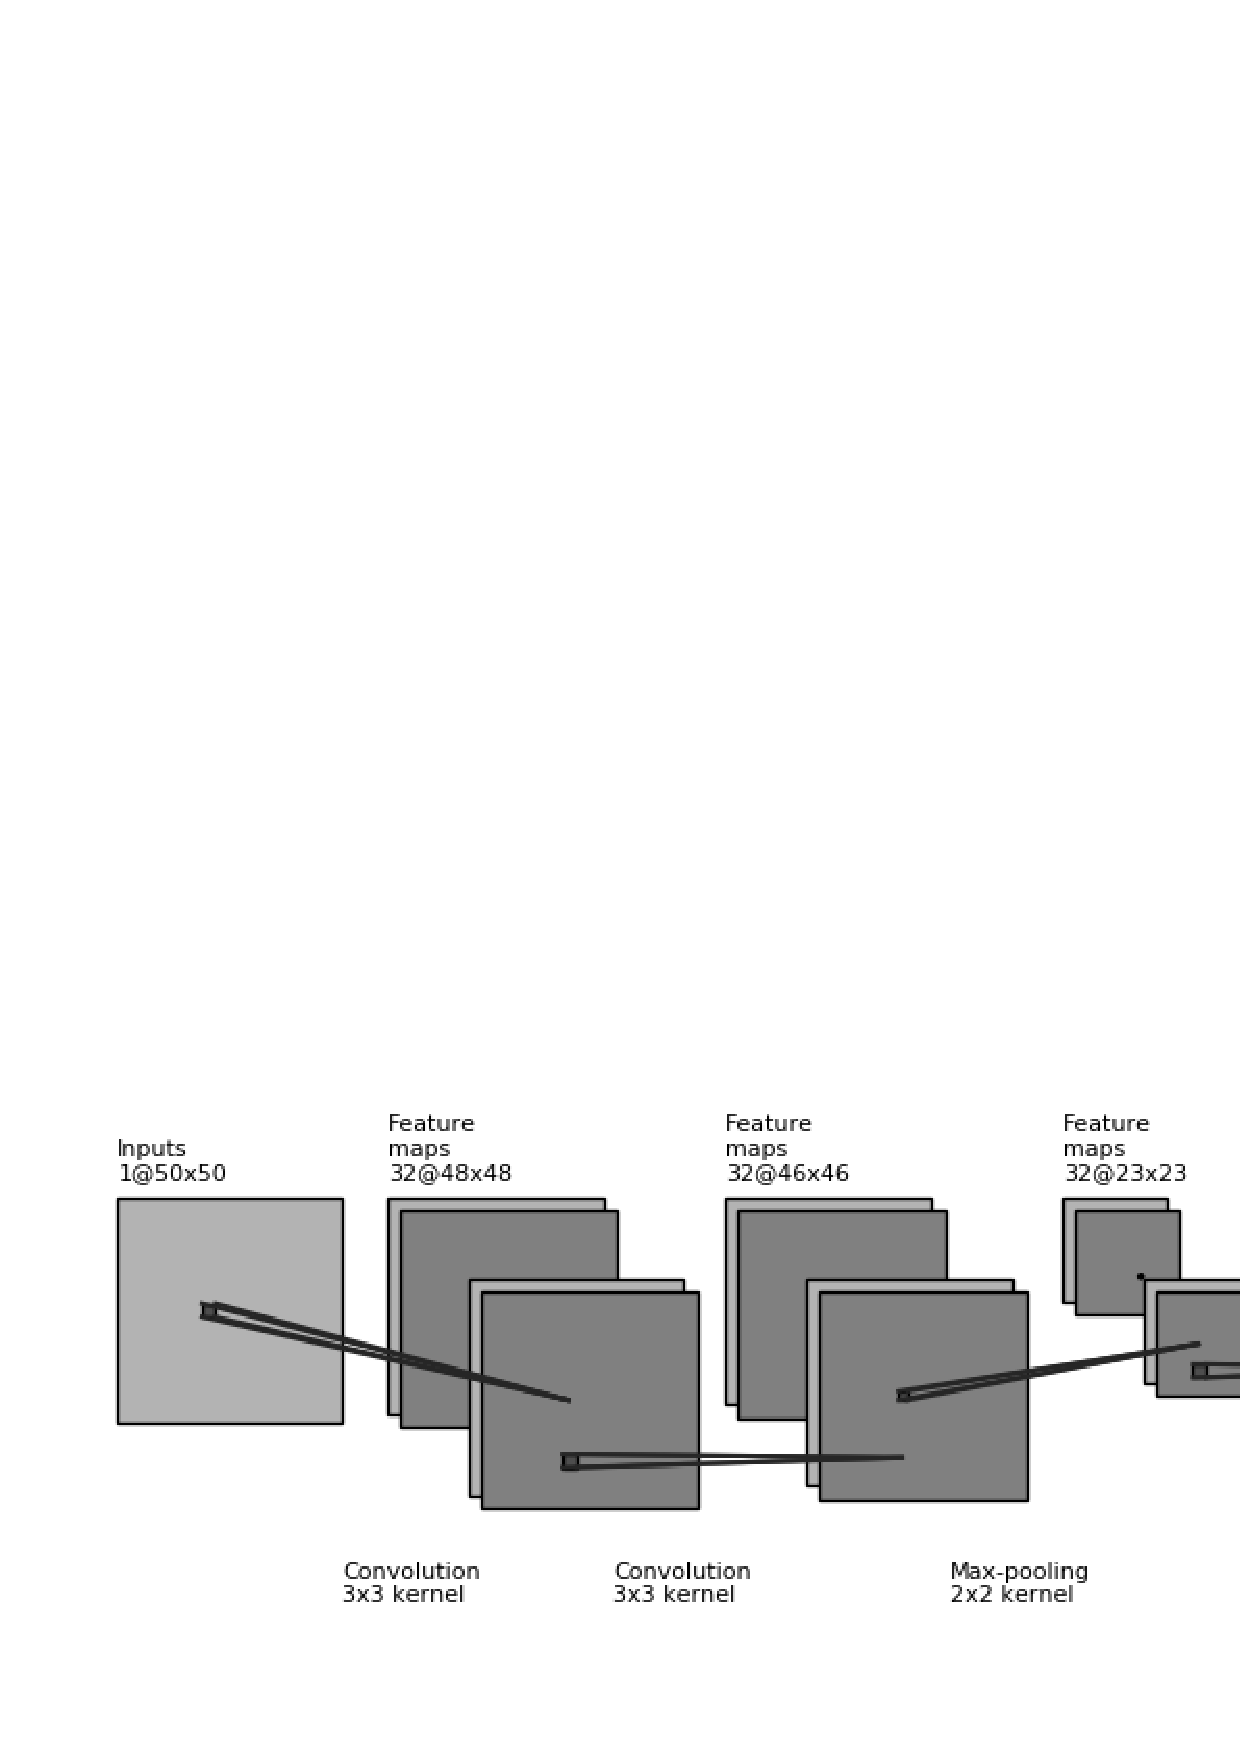
\includegraphics[scale=0.4]{mynet.png}
    \caption{网络结构示意}
    \label{fig:label}
\end{figure}
spp层是使用了动态尺寸的池化核将任意尺寸的输入池化到固定尺寸的输出。首先需要一个$BINS$来决定输出的尺寸,通常会选择多个输出尺寸来获得更多的信息。如输入图片尺寸为$x \times x$,需要的输出尺寸为$n \times n$,则计算
$$ksize = \lceil \frac x n \rceil$$
$$stride = \lfloor \frac x n \rfloor$$
再利用$ksize$和$stride$做最大池化。对$BINS$中每个输出尺寸都做了最大池化后,把这些数据排成一行输出到全连接层。\cite{spp}最开始是为了实现输入不同尺寸的图片到网络中进行训练所以想使用spp,但由于tensorflow的局限,一是如果输入不同尺寸的图片,就没法使用batch,只能每次输入一个图片;二是spp需要使用图片的动态尺寸,生成动态池化核来进行池化,但tensor自带的池化函数只支持静态池化核,需要自己重写池化函数,又遇到了使用tensor写循环语句的困难。考虑到图片伸缩对本问题的影响不大,故最后改为将输入单词图片都resize到$50 \times 50$,但仍然保留spp层。尽管spp层也需要每次输入的图片尺寸相同,但如果输入图片都变为另外一个尺度,网络也不需要改动,可以直接利用原网络。这样就可以实现多尺度维度的输入来提高效果。

\section{结果分析与改进}

\subsection{网络训练结果}
\noindent

使用了如上网络,以100大小的batch进行了50000次训练。训练集共有含过采样的100万张单词图片,测试集为无过采样的1万张单词图片。测试结果评估采用了4个指标,accuracy、precision、recall、F1 Measure。TP为预测正确的正类,FP为预测错误的正类,TN为预测正确的负类,FN为预测错误的负类。accuracy为所有图片预测正确的概率,precision为预测为正类的图片中预测正确的比例,recall为所有正类中被预测正确的比例,F1为precision和recall的调和平均。
\[accuracy = \frac {TP + TN} {TP + FP + TN + FN}\]
\[precision = \frac {TP} {TP + FP}\]
\[recall = \frac {TP} {TP + FN}\]
\[F_1 = \frac {2 TP } {2 TP + FP + FN}\]



在训练集的4个不同位置取一万张图片,以及在测试集上分别计算accuracy、precision、recall、F1 Measure,结果如下表。使用formula\_find.py进行实际效果查看,错误率较高的在于一些短单词,如the、and、of等。对于被分割的公式,在重建时直接将相邻的被预测为公式的单词合并起来,然后用红框标注。发现在测试集上precision明显下降,因为测试集没有过采样,所以非公式图片比公式图片多很多,故有更大比例的非公式图片被识别为公式图片,故precision下降了。也有可能是训练结果过拟合导致的。

\begin{figure}[hp]
\centering
\begin{tabular}{ccccc}
\toprule
Set& accuracy& precision& recall& F1\\
\midrule
Train set 1& 0.83& 0.88& 0.76& 0.82\\
Train set 2& 0.84& 0.87& 0.80& 0.83\\
Train set 3& 0.80& 0.90& 0.67& 0.77\\
Train set 4& 0.79& 0.88& 0.69& 0.78\\
Test set& 0.83& 0.47& 0.72& 0.57\\
\bottomrule
\end{tabular}
\end{figure}

每1000次训练将模型在测试集上进行检测,得到accuracy、precision、recall、F1 Measure的变化趋势。除最开始明显上升外,整体有波动,稳定在一定范围内。

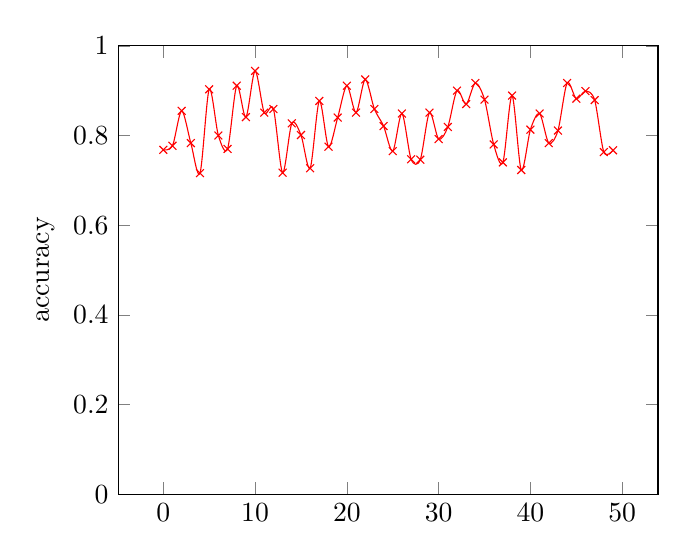
\begin{tikzpicture}
    \begin{axis}[ymin=0, ymax=1,
        ylabel=accuracy]
    \addplot+[smooth, color=red, mark=x]                    % 设置绘图的类型是光滑线图
    coordinates
    {
        (0, 0.7680000066757202) (1, 0.7770000100135803) (2, 0.8550000190734863) (3, 0.7829999923706055) (4, 0.7160000205039978) (5, 0.902999997138977) (6, 0.800000011920929) (7, 0.7699999809265137) (8, 0.9110000133514404) (9, 0.8410000205039978) (10, 0.9440000057220459) (11, 0.8510000109672546) (12, 0.859000027179718) (13, 0.7170000076293945) (14, 0.8270000219345093) (15, 0.8009999990463257) (16, 0.7269999980926514) (17, 0.8769999742507935) (18, 0.7749999761581421) (19, 0.8399999737739563) (20, 0.9110000133514404) (21, 0.8510000109672546) (22, 0.925000011920929) (23, 0.859000027179718) (24, 0.8209999799728394) (25, 0.7649999856948853) (26, 0.8489999771118164) (27, 0.746999979019165) (28, 0.7459999918937683) (29, 0.8510000109672546) (30, 0.7919999957084656) (31, 0.8190000057220459) (32, 0.8999999761581421) (33, 0.8700000047683716) (34, 0.9169999957084656) (35, 0.8799999952316284) (36, 0.7799999713897705) (37, 0.7400000095367432) (38, 0.8889999985694885) (39, 0.7229999899864197) (40, 0.8130000233650208) (41, 0.8489999771118164) (42, 0.7829999923706055) (43, 0.8109999895095825) (44, 0.9169999957084656) (45, 0.8820000290870667) (46, 0.8989999890327454) (47, 0.8790000081062317) (48, 0.7630000114440918) (49, 0.7670000195503235)
    };
    \end{axis}
\end{tikzpicture}


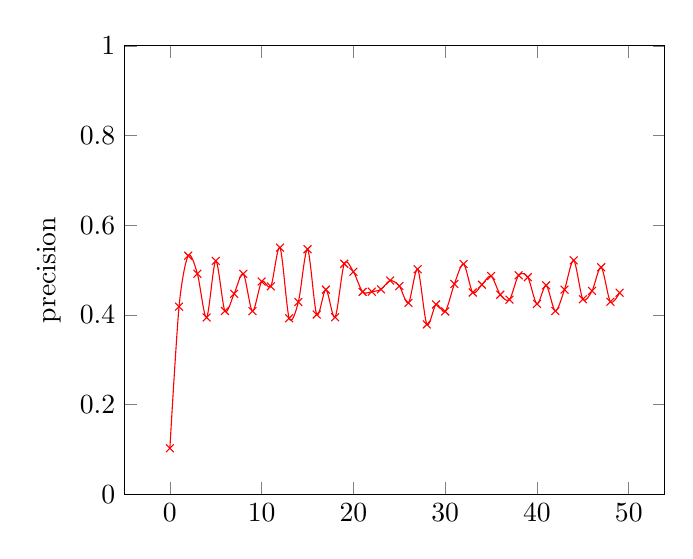
\begin{tikzpicture}
    \begin{axis}[ymin=0, ymax=1,
        ylabel=precision]
    \addplot+[smooth, color=red, mark=x]                    % 设置绘图的类型是光滑线图
    coordinates
    {
        (0, 0.10227267450940637) (1, 0.4181817318844488) (2, 0.531791767957752) (3, 0.4914528961028762) (4, 0.39402169052022534) (5, 0.5202701106741453) (6, 0.40856023911048184) (7, 0.44680845668863683) (8, 0.4913791180295048) (9, 0.4080716658007849) (10, 0.4742265821664585) (11, 0.4634145315171357) (12, 0.5497834417310405) (13, 0.3923705236686806) (14, 0.42857135344745423) (15, 0.546255397357019) (16, 0.4005681301540768) (17, 0.45614022977348306) (18, 0.39455776220103844) (19, 0.5138888078801535) (20, 0.4959998198531441) (21, 0.45116269542904797) (22, 0.4516127378775276) (23, 0.45673066954067154) (24, 0.4763778676081821) (25, 0.4641743891791755) (26, 0.42672405442568057) (27, 0.5015872292951588) (28, 0.3786126670838483) (29, 0.42307683073241154) (30, 0.4074073389027238) (31, 0.46885238922667033) (32, 0.5133331779647318) (33, 0.44973534170395274) (34, 0.4671531298633628) (35, 0.4864863372537463) (36, 0.44478521413123473) (37, 0.43380276142362) (38, 0.48809510619355034) (39, 0.4838709033205131) (40, 0.4242423512857085) (41, 0.46575332810425396) (42, 0.40845063893087913) (43, 0.4560810111282234) (44, 0.5214284023370511) (45, 0.43478248609258174) (46, 0.4534160212108353) (47, 0.5060239579912521) (48, 0.4289854507944657) (49, 0.4491017353617148)
    };
    \end{axis}
\end{tikzpicture}

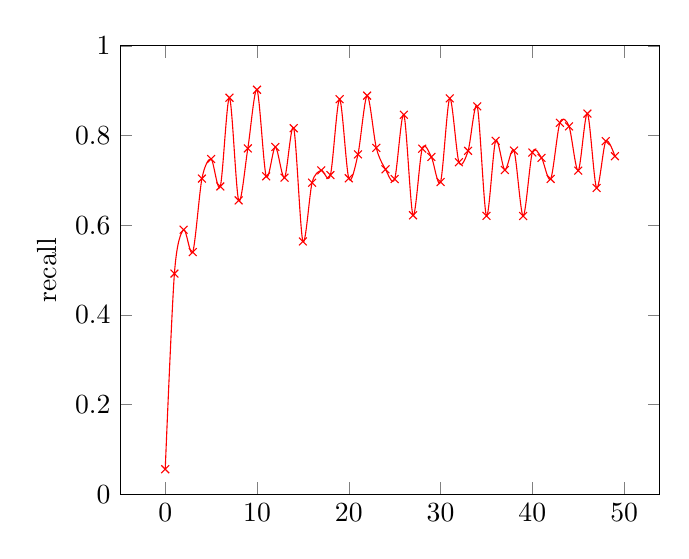
\begin{tikzpicture}
    \begin{axis}[ymin=0, ymax=1,
        ylabel=recall]
    \addplot+[smooth, color=red, mark=x]                    % 设置绘图的类型是光滑线图
    coordinates
    {
        (0, 0.05555553998631103) (1, 0.49197849018294704) (2, 0.5897434181133989) (3, 0.5399059882080096) (4, 0.7038833400181834) (5, 0.7475724860219577) (6, 0.6862743061646712) (7, 0.8842103150363884) (8, 0.6551720718992409) (9, 0.771186143967824) (10, 0.9019599813937293) (11, 0.7089549836827875) (12, 0.7743900295289454) (13, 0.7058821958480288) (14, 0.8161761981298377) (15, 0.5636362473225179) (16, 0.6945811254485994) (17, 0.7222219186219965) (18, 0.7116562435021873) (19, 0.88095214288592) (20, 0.7045450910647995) (21, 0.75781223121389) (22, 0.8888882483259677) (23, 0.7723574384961508) (24, 0.7245507012302338) (25, 0.7028300381677623) (26, 0.8461535178178609) (27, 0.6220471329098577) (28, 0.7705880295021034) (29, 0.752136460282543) (30, 0.6962023315978674) (31, 0.8827158020047197) (32, 0.7403842921788956) (33, 0.7657654525612815) (34, 0.8648643342597293) (35, 0.6206894122477955) (36, 0.7880432838200557) (37, 0.723004540730726) (38, 0.7663548150237872) (39, 0.6203006460090009) (40, 0.7619045265958367) (41, 0.7499997496328238) (42, 0.7030301095908024) (43, 0.8282206282137524) (44, 0.8202243006952176) (45, 0.7216491467750457) (46, 0.8488367611961705) (47, 0.6829265771965964) (48, 0.787233852444885) (49, 0.7537686722560564)
    };
    \end{axis}
\end{tikzpicture}
    
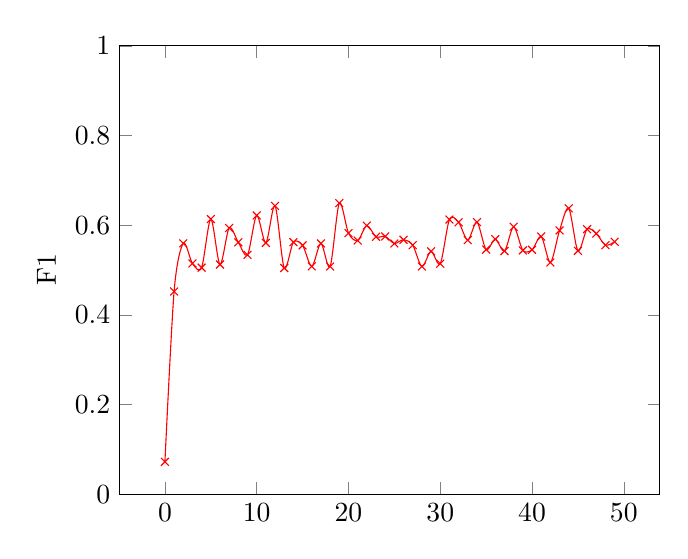
\begin{tikzpicture}
    \begin{axis}[ymin=0, ymax=1,
        ylabel=F1]
    \addplot+[smooth, color=red, mark=x]                    % 设置绘图的类型是光滑线图
    coordinates
    {
        (0, 0.0719999869248226) (1, 0.45208840165901304) (2, 0.5592704395415238) (3, 0.5145413347647865) (4, 0.50522644087588) (5, 0.6135457057572432) (6, 0.5121950652350732) (7, 0.593639528354783) (8, 0.5615762290861016) (9, 0.5337242691171721) (10, 0.6216214309353425) (11, 0.5604719013410473) (12, 0.6430379007749987) (13, 0.504378243609918) (14, 0.5620252518584634) (15, 0.5548097870507263) (16, 0.5081080665440171) (17, 0.5591396939609217) (18, 0.5076585928935132) (19, 0.6491227423900725) (20, 0.5821595003286365) (21, 0.5655975927752449) (22, 0.5989303358748921) (23, 0.5740180481559545) (24, 0.5748217907437793) (25, 0.5590993895251913) (26, 0.5673351697507826) (27, 0.5553602368834522) (28, 0.5077518933102708) (29, 0.5415383858898317) (30, 0.5140186370644626) (31, 0.6124196406770692) (32, 0.6062991042285955) (33, 0.5666665809112568) (34, 0.6066349405631104) (35, 0.5454544516530538) (36, 0.5686274003614823) (37, 0.5422534777847363) (38, 0.5963635379095901) (39, 0.54365729047446) (40, 0.5450121052469311) (41, 0.5746478138338862) (42, 0.5167037339458502) (43, 0.5882352359349926) (44, 0.6375544587557744) (45, 0.5426355634278431) (46, 0.5910930087628296) (47, 0.5813147875721435) (48, 0.5553470446290492) (49, 0.5628517344213336)
    };
    \end{axis}
\end{tikzpicture}

\subsection{分析与改进}
\noindent

网络结果不尽如人意,对于原因有如下分析。

一是在数据上。数据过于简单,特别是过采样部分,直接使用了复制原图片的方式进行过采样,缺乏变化。单词图片之间也有很大差异,寻找共性特征比较困难,故长单词一般很好地被区分,但短单词却容易和公式混淆。而且公式内也有许多字母符号,与某些非公式单词可能难以分别。实际上短单词也容易被误认为是公式,尤其是and、of。对于单词the,在测试时发现同一张论文图片中,有的the被认为是公式,有的被认为是单词,于是将这些the单独提取出来,发现只有图片的高度不同,高度高一点的被认为是公式,高度低一点的被认为是单词,这也是由于数据本身的多样性不足。

二是在参数初始化上,直接使用了截断正态分布来初始化权重,可能会对结果造成影响。

三是网络结构上。这次采用的网络结构主要是根据自身条件进行的舍取,缺乏有效性的验证。

根据以上的错误分析,可以有如下的改进。在数据预处理上,采用最小二乘法的单词分割虽然效果还不错,但还不够精确,特别是容易将公式分割开。不过,如果仍然采用以空格为依据的单词分割,这一点比较难改进,有的公式内部确实有较大的空格,与单词间空格难以区分,但可以尝试精细的调参,提高表现,还可以使用去掉一些较小值后再进行最小二乘法,使结果更偏离小宽度空白。在过采样时,应该使用更多样化的采样,如使用SMOTE算法进行过采样。SMOTE算法是将少数类样本取k临近样本并在两个样本间做一个随机的平移。由于网络使用了spp层,还可以考虑将输入图像resize到更多尺度的数据做多尺度的训练。在参数初始化上,可以采用MSRA初始化,即权值初始化为服从方差为$\frac 2 n$的高斯分布。\cite{msra}网络结构上应该测试更多的模型,并在通过验证集调节超参数,对网络的深度、学习率、核尺寸等进行进一步的调节。

\subsection{CTPN}
\noindent

\begin{figure}[hp]
    \centering
    
\includegraphics[scale=0.5]{rpn.png}
    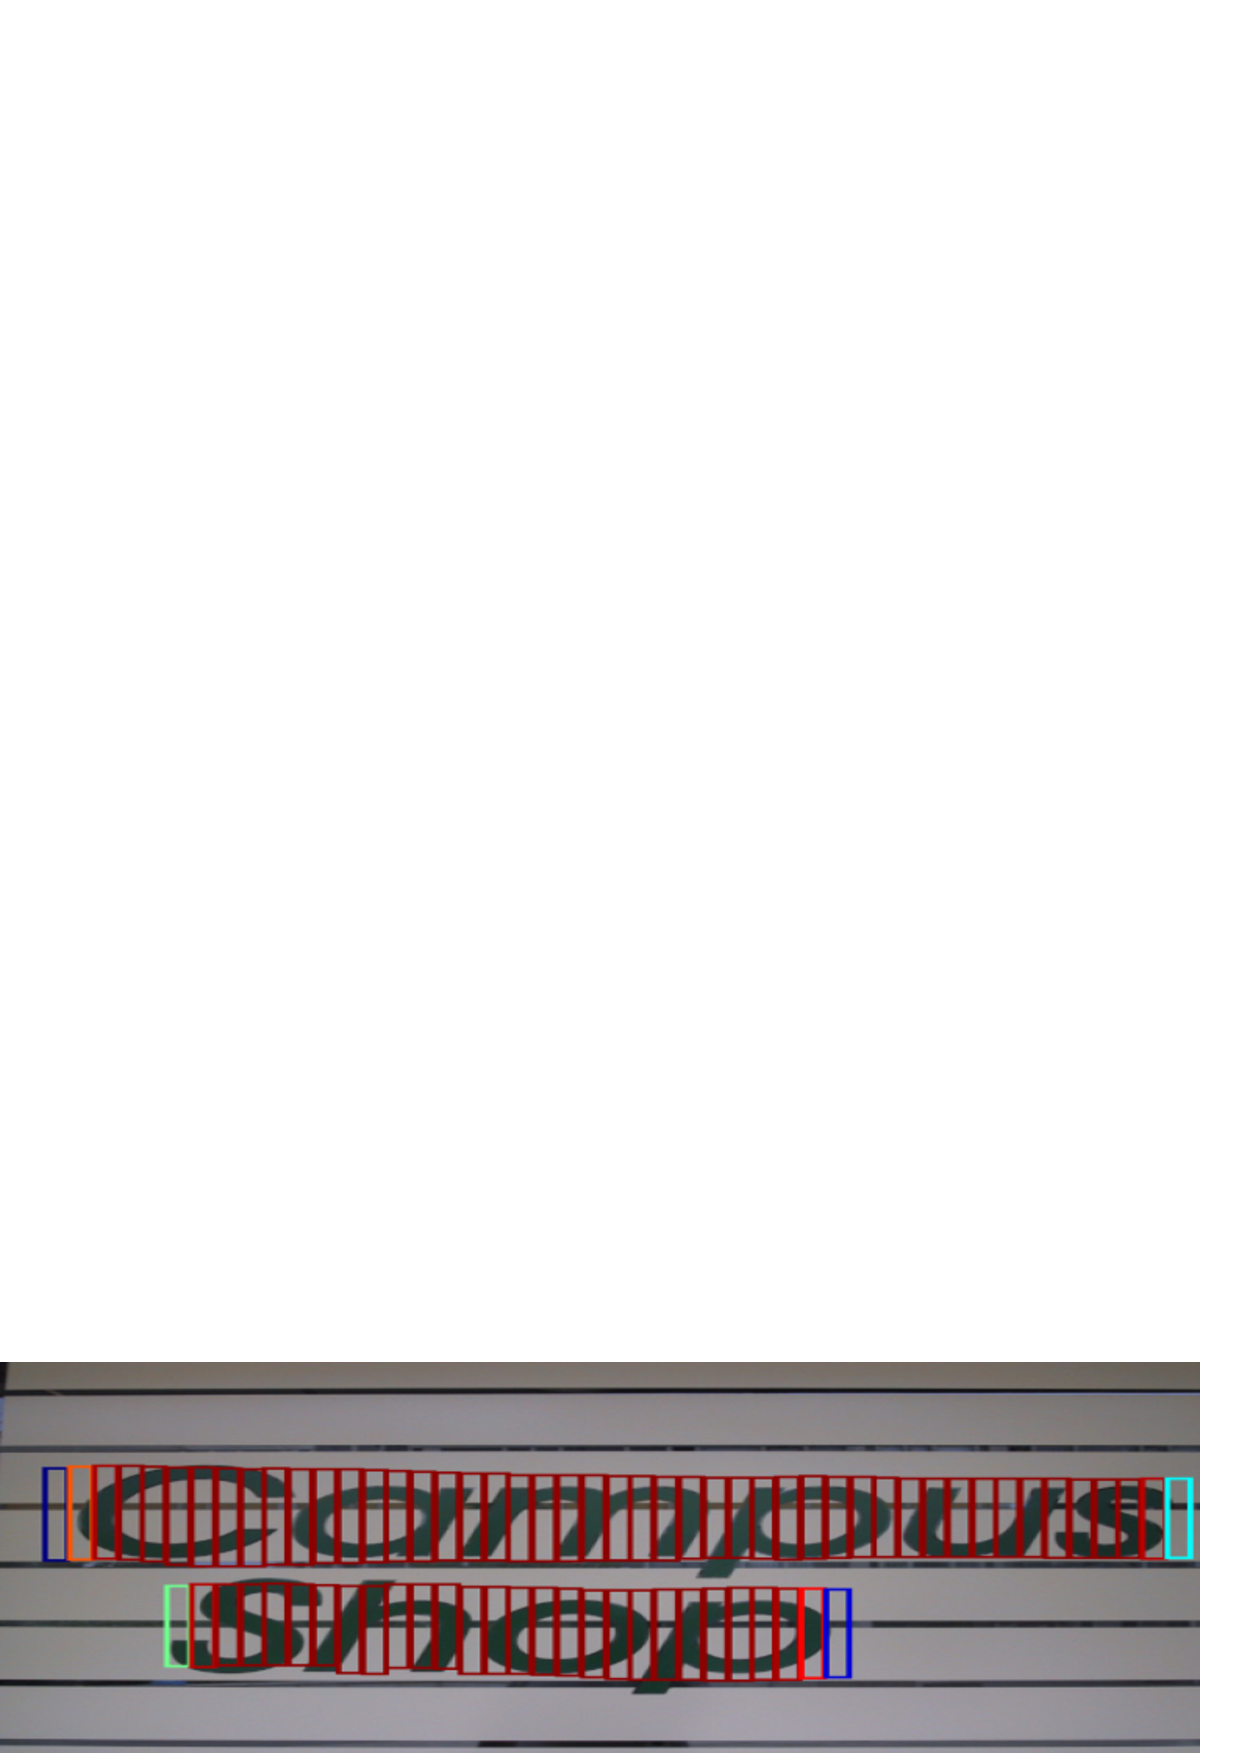
\includegraphics[scale=0.5]{ctpn.png}
    \caption{CTPN proposals}
    \label{fig:label}
\end{figure}

在独立做完以上工作后,查阅论文时发现在OCR领域已有许多类似的工作。传统的做法即是先做单词分割,再使用分类器进行分割。如CTPN\cite{ctpn}、CRNN等。CRNN主要做的是文字识别工作,而CTPN做的是文字检测。

CTPN做的是自然场景图象中的水平文字检测,主要是在Faster RCNN的基础上结合LSTM生成的模型。首先是通过VGG提取特征,将生成的feature map经过一些处理后输入双向LSTM中,生成既包含CNN学习到的空间特征,也包含LSTM学习到的序列特征的特征图。再将特征图通过类似Faster RCNN的RPN网络,获得text proposals。CTPN生成的是宽度不变的anchor,通过寻找anchor中心和高度来获得一个小尺寸的text proposal,如图2,上面是传统的RPN的输出,下面为CTPN输出的text proposals,可以看见一个文本有许多小宽度的proposals,接下来只需要通过文本线构造办法,将这些连接起来形成一个文本检测框。

CTPN的工作是自然场景图象中的文字检测,用在我们的论文图片中有大材小用的样子。但是CTPN的方法给予了我一些启发。在处理单词图片时我们直接将单词图片resize到了固定长宽,如果我们不是resize,而是以一定宽度做crop,甚至以字母图片为基础来进行训练,同时在网络中引入RNN来获得序列信息,对效果也许会有提升。

\bibliography{ref.bib}
\end{document}
